\subsection{Reprezentace znalostí}
Pro porovnání obrázku s jeho popisem v přirozené řeči bylo nutné zvolit či navrhnout nějakou formu reprezentace znalostí,
která by umožnila zachytit sémantiku z obou zdrojů.
Jak již bylo výše zmíněno, zvolen byl expertní přístup a to v tomto případě znamená, že referenční popis obrázku je vytvořen lidským expertem,
což klade další omezení na formát reprezentace znalostí.

Při návrhu bylo tedy potřeba brát v úvahu následující požadavky a najít nějaký formát, který by představoval vhodný kompromis mezi nimi.
\begin{itemize}
	\item \textbf{Čitelnost člověkem}:\\
	      Aby byl lidský expert schopen vytvořit, číst a případně upravit referenční popisy,
	      je nutné, aby byl schopen porozumět formě a zápisu uložených dat.
	      Toto omezení tedy upřednostňuje textové formáty a prakticky vyřazuje binární data.

	      Výjimku by mohl tvořit nějaký binární formát s přidruženým editorem,
	      kde by člověk mohl v grafickém prostředí prohlížet a manipulovat data, ale takový případ je nad rámec této práce.
	\item \textbf{Kompaktnost a struktura dat}:\\
	      Dalším důležitým aspektem je struktura a kompaktnost dat.
	      Pomocí počítače je poměrně snadné v krátkém čase zpracovat velké množství jednoduchých datových záznamů,
	      nicméně člověk se bude lépe orientovat v nějakém kompaktnějším popisu, který ačkoli může být složitější ve své struktuře,
	      tak bude pro člověka lépe názorný a uchopitelný.
	\item \textbf{Univerzálnost formátu}:\\
	      Podstatnou vlastností pro hledanou reprezentaci znalostí je její schopnost zachytit popis různých obrázků.
	      Navržený formát tedy musí být dostatečně univerzální, aby pomocí něj šlo popsat co nejširší spektrum informací,
	      od jednoduchých obrázků zobrazujících například jeden statický objekt, přes složitější obrázky zobrazující více objektů,
	      až po dynamické komplexní scény zobrazující mnoho objektů, činnosti a vazby mezi nimi.
	\item \textbf{Počítačová zpracovatelnost}:\\
	      V neposlední řadě je také potřeba dbát na to, aby navržený formát bylo možné co nejsnadněji zpracovat programově, na počítači.
	      Dynamické formáty s volnou strukturou bývají složitější na strojové zpracování, než fixní formáty s přesně definovanou podobou.
\end{itemize}

% TODO: přidat info o tom, že expertní přístup k referenčním popisům dává absolutní kontrolu nad obsahem 
%       a protože stačí referenční popis udělat jednou a pak se jenom používá, tak to tolik nevadí, že to musí psát člověk
%       možná to formulovat stylem "protože referenční popis stačí udělat jednou, ale pořádně, tak je lepší aby ho udělal člověk-expert, než automat"

S ohledem na tyto body byla navržena reprezentace znalostí založená na sémantických sítích, která definuje 4 základní aspekty popisu: objekty, jejich hierarchii,
statické atributy a dynamické vazby.
Detailnější popis těchto jednotlivých aspektů je v následujících částech, spolu s ukázkami na konkrétních příkladech a obrázcích.
% TODO: Slibuji příklady, tak bych je měl přidat a nebo slib odstranit.

% TODO: jak s anglikanismy?
% TODO: jak a kde použít \emph pro "objekt"? 
\subsubsection*{Objekty ve scéně}
\newcommand{\objekt}{{\color{red!70!black}\texttt{objekt}}}
Cokoli, co lze v obrázku ohraničit rámečkem (angl.~bounding-box) a při separaci od zbytku scény (obrázku) neztratí nebo zásadně nezmění svůj význam,
lze považovat za \emph{objekt}.

Jako \emph{objekt} v obrázku lze tedy označit zobrazené fyzické předměty, postavy, zvířata, ale také nehmotné pojmy jako \enquote{nebe},
místa, lokace či místnosti (např.~\enquote{kuchyň} nebo \enquote{louka}) a části jiných objektů (např.~\enquote{obličej} jsou součást hlavy nebo celého člověka).

% TODO: vyměnit dlouhé popisy za jeden ukázkový příklad? Ilustrace farmy se zvířaty a nářadím/stodolou by mohla fungovat dobře.
Tato definice objekt u byla záměrně navržena velmi obecně, aby byl definovaný formát univerzální a šel použít i pro popis velmi odlišných obrázků s různými účely.
Potenciální nevýhodou, která plyne z univerzálnosti formátu, může být v některých situacích problém nejednoznačnosti.

V jednom obrázku lze definovat různé množiny objektů, podle toho, jak moc detailní popis expert vytvoří.
Například pokud by byl na obrázku člověk, lze jej popsat jedním objektem jako \enquote{člověk} nebo \enquote{osoba},
ale také by šlo definovat ještě mnoho dalších objektů, například pro jednotlivé části těla nebo oblečení.

Kromě různých úrovní detailů lze také na problematiku nejednoznačnosti narazit v situaci, kdy je pro nějaký (dostatečně komplexní) obrázek
možné sestavit různé množiny objektů podle toho, pro jaké potřeby je zrovna obrázek a referenční popis používán.
Pro aplikaci, kde je podstatné zachycení živých objektů, může být množina objektů v referenčním popise tvořena lidmi či zvířaty.
Pro jiné použití pak ale může být podstatné zachytit prostředí a neživé předměty,
takže množina objektů by byla tvořena částmi prostředí (např.~stromy, křoví, voda, skály), budovami nebo obecnými předměty.

\subsubsection*{Hierarchie objektů}
Kromě množiny samotných objektů lze v obrázku také definovat jejich hierarchii.
To přirozeně plyne z výše zmíněné definice \emph{objektu}, která umožňuje specifikovat část existujícího objektu jako další samostatné objekty.

Příkladem takového popisu může být například situace, kdy je na obrázku strom.
Strom je možné rozdělit na korunu a kmen, korunu pak je možné dále dělit na větve.
Schématicky lze tento popis znázornit jako stromovou strukturu, viz Obrázek~\ref{fig:schema_hierarchie_objektu}.
\begin{figure}[ht!]
	\centering
	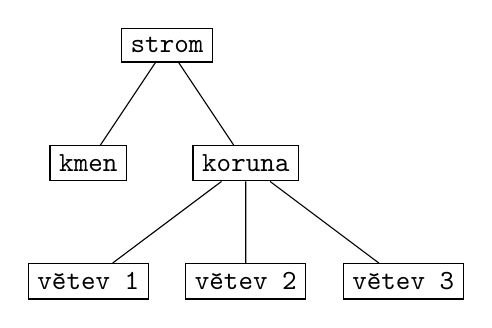
\begin{tikzpicture}[sibling distance=20mm]
		\node[draw, rectangle] {\texttt{strom}}
		child {node[draw, rectangle] {\texttt{kmen}}}
		child {node[draw, rectangle] {\texttt{koruna}}
				child {node[draw, rectangle] {\texttt{větev 1}}}
				child {node[draw, rectangle] {\texttt{větev 2}}}
				child {node[draw, rectangle] {\texttt{větev 3}}}
			}
		;
	\end{tikzpicture}
	\caption{Schématické znázornění hierarchie objektů}\label{fig:schema_hierarchie_objektu}
\end{figure}

Z pohledu daného objektu jsou \enquote{vyšší} (obecnější) objekty označované jako \emph{rodičovské objekty} (nebo jen \emph{rodiče}) a
\enquote{nižší} (konkrétnější) objekty pak jako \emph{potomci}.
Aby byl popis jednoznačný, tak bylo rozhodnuto, že vazby musejí být definované v referenčním popisu oboustranně.
Tím je myšleno to, že pokud objekt \texttt{\color{red!80!black}A} specifikuje objekt \texttt{\color{red!80!black}B} jako svého rodiče,
pak musí i objekt \texttt{\color{red!80!black}B} specifikovat \texttt{\color{red!80!black}A} jako svého potomka.
Pokud je hierarchická vazba definována pouze jednostranně, měl by být referenční popis implementací systému odmítnut jako invalidní.

Možnost definovat hierarchii objektů nabízí mimo jiné také způsob, jak vytvořit skupiny objektů, které k sobě nějakým způsobem patří.
Například strom může být součástí lesa, kráva může být součástí stáda nebo postava na hřišti může být součástí fotbalového týmu.
Tato příslušnost objektu nějaké skupině je dalším typem sémantické informace, kterou umožňuje navržený formát zachytit bez nutnosti definovat další specializované struktury.

Mohou však nastat situace, kdy je potřeba jeden objekt zařadit do několika různých skupin.
Z tohoto důvodu bylo rozhodnuto, že každý objekt může mít libovolné množství rodičů a libovolné množství potomků.
% TODO: zdůvodňovat? dávat příklad? přirovnávat k OOP dědičnost vs kompozice (případně zmínit flaws of inheritance)?

\subsubsection*{Statické atributy objektů}
% TODO:
% 1. dává smysl, že když máme objekty, chceme popsat jejich vlastnosti
% 2. jako atributy jsem označil ty informace, které nejsou závislé na jiných objektech - typicky vlastnosti nebo samostatné činnosti, například barva nebo "plave"
% 3. příklad?

\subsubsection*{Dynamické vazby mezi objekty}
% TODO:
% 1. mezi objekty existují vazby, které je taky potřeba popsat -> to je poslední kousek sémantické informace co můžeme chtít zachytit (?)
% 2. k popisu informací týkajících se vzájemně dvou objektů jsem definoval "vazby" (triplety)
% 3. příklad?
